%%%%%%%%%%%%%%%%%%%%%%%%%%%%%%%%%%%%%%%%%%%%%%%%%%%%%%%%%%%%%%%%%%%%%%%%%%%%%%%%%%
%%%%%%%%%%%%%%%%%%%%%%%%%%%%%%%%%%%%%%%%%%%%%%%%%%%%%%%%%%%%%%%%%%%%%%%%%%%%%%%%%%
\section{MIP-DSA Solves Based on Algebraic Multigrid Techniques} \label{sec_amg}
%%%%%%%%%%%%%%%%%%%%%%%%%%%%%%%%%%%%%%%%%%%%%%%%%%%%%%%%%%%%%%%%%%%%%%%%%%%%%%%%%%
%%%%%%%%%%%%%%%%%%%%%%%%%%%%%%%%%%%%%%%%%%%%%%%%%%%%%%%%%%%%%%%%%%%%%%%%%%%%%%%%%%

%%%%%%%%%%%%%%%%%%%%%%%%%%%%%%%%%%%%%%%%%%%%%%%%%%%%%%%%%%%%%%%%%%%%%%%%%%%%%%%%%%
\subsection{Principles}
%%%%%%%%%%%%%%%%%%%%%%%%%%%%%%%%%%%%%%%%%%%%%%%%%%%%%%%%%%%%%%%%%%%%%%%%%%%%%%%%%%

As mentioned above, a common way to solve a SPD system of equations is to use
conjugate gradient preconditioned with SSOR (PCG-SSOR). In this research, we
will compare the calculation time and the number of iterations using conjugate 
gradient preconditioned with Symmetric Gauss-Seidel (PCG-SGS), which is PCG-SSOR with a
damping factor of one, to those of CG preconditioned with an
algebraic multigrid method. PCG-SGS was chosen because little difference was noted 
when employing other damping factors \cite{wang_personal_comm}. In \cite{amg_pn}, the authors 
used an algebraic multigrid method to precondition the Krylov solver for the 
even-parity finite element-spherical harmonics (FE-$P_N$) method. The AMG 
preconditioner resulted in a 60\% reduction in the solution time compared to 
ILU(0) preconditioning and even more reduction compared to SSOR preconditioning. 
In our implementation, we have linked our code to the ML package 
\cite{ml_guide} from the Trilinos library and the AGMG code \cite{agmg_guide}. 
ML is a multigrid preconditioning package that uses a smoothed aggregation 
algebraic multigrid to build a preconditioner for a Krylov method. AGMG is an 
aggregation-based algebraic multigrid code written in Fortran 90.
%
The first multigrid methods developed were geometric multigrid techniques, used as 
stand-alone solvers. In many applications, they achieve the so-called 
``textbook multigrid efficiency'', i.e., ``the solution to the governing 
system of equations [is attained] in a computational work that is a small 
multiple of the operation counts associated with discretizing the system'' 
\cite{textbook_eff}. However, in many other applications, multigrid methods, 
and particularly algebraic multigrid methods, cannot achieve such efficiency 
\cite{k_cycle} and, in such cases, they are often used as preconditioner for 
Krylov subspace methods. 

Before describing a general multigrid method, we recall the process using a 
two-grid method. Assume one wants to solve the following system:
\begin{equation}
  \bs{A}_f u_f = b_f,
\end{equation}
defined on a fine grid $\Gamma_f$. The two-grid algorithm is given by:
\begin{enumerate}
  \item Perform $\nu_1$ pre-smoothing iterations using a smoother (Jacobi,
    Gauss-Seidel or ILU) and an initial guess $u_0$: $u = S^{\nu_1}(u_0,b_f)$
  \item Compute the residual on the fine grid $\Gamma_f$ and restrict it to
    the coarse grid $\Gamma_c$: $r_c = \bs{R}(b_f-\bs{A}_f u)$;
  \item Solve the system on the coarse grid: $v=\bs{A}_c^{-1} r_c$;
  \item Interpolate the coarse grid correction to the fine grid and add the
    correction to $u$: $u=u+\bs{P}v$;
  \item Perform $\nu_2$ post-smoothing iterations: $u = S^{\nu_2}(u,b_f)$.
\end{enumerate}
When using AMG, the matrix $\bs{A}_c$ on the coarse grid is given by the
Galerkin approximation:
\begin{equation}
  \bs{A}_c = \bs{R} \bs{A}_f \bs{P},
\end{equation}
where $\bs{P}$ is a prolongation matrix and $\bs{R}$ is a restriction matrix. 
Generally, solving the system $\bs{A}_c v = r_c$ on the coarse grid is still
quite expensive, therefore this step is recursively replaced by $n_{\gamma}$
sequences of the two-grid method until the system can be efficiently inverted 
with a direct solver.
%This yields the multigrid method. 
When $\gamma = 1$, respectively $\gamma =
2$, the multigrid method is said to use a $V-$cycle, respectively a $W-$cycle. 
In \Cref{fig_v_w}, a dot represents a smoothing operation and a square a
direct inversion. The grid transfer operators are symbolized by lines.
\begin{figure}[H]
  \centering
  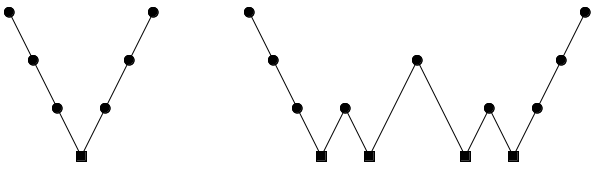
\includegraphics[width=0.5\textwidth]{v_w_cycles}
  \caption{$V-$ and $W-$cycles.}
  \label{fig_v_w}
\end{figure}

The main difference between geometric and algebraic multigrid techniques
pertains to the method used
to coarsen the grid. Algebraic multigrid methods only use the properties of the
matrix. Among the algebraic multigrid methods, there are three main categories: 
the classical Ruge-Stueben AMG, the plain aggregation AMG, and the
smoothed aggregation AMG. ML uses smoothed aggregation AMG and AGMG
uses plain aggregation AMG. Next, we briefly explain the coarsening step in
the ML and AGMG implementations. The coarsening step is the most important 
step because if the coarsening occurs too fast, convergence rates will 
decrease. However, if the coarsening is too slow, more memory may be 
required to solve the problem. 

%%%%%%%%%%%%%%%%%%%%%%%%%%%%%%%%%%%%%%%%%%%%%%%%%%%%%%%%%%%%%%%%%%%%%%%%%%%%%%%%%%
\subsection{ML Package of Trilinos}
%%%%%%%%%%%%%%%%%%%%%%%%%%%%%%%%%%%%%%%%%%%%%%%%%%%%%%%%%%%%%%%%%%%%%%%%%%%%%%%%%%
When using a smoothed aggregation scheme, the smoothed interpolation operators,
$\bs{P}_k$, are the transpose of the coarsening operators,
$\bs{R}_k=\bs{P}_k^T$. Therefore, when the $\bs{P}_k$ matrices are built, the
coarsening operator is also known. First, the graph of the matrix is
constructed: if element $(i,j)$ or $(j,i)$ of the matrix is non-zero, an edge
is built between the vertex $i$ and the vertex $j$ \cite{ml_guide}. Second,
the vertices are 
aggregated. When using ML on a single processor, two aggregation schemes can
be used: the uncoupled scheme or the maximally independent sets (MIS) scheme. 
The uncoupled scheme tries to build aggregates of size $3^d$ where $d$ is the
dimension of the problem; its algorithm proceeds as follows \cite{mis}:
\begin{description}
  \item[Step 1:] As long as there are points not adjacent to an aggregate:
    \begin{enumerate}
      \item Choose a point which is not an adjacent to an
        aggregate. This point is a new root point.
      \item Define a new aggregate as the root point and its neighbors 
    \end{enumerate}
  \item[Step 2:] Add all the points left to the existing aggregates or form 
    new aggregates with them.
\end{description}
The MIS scheme used in ML applies the MIS algorithm \cite{graph_coloring} to
the graph of the matrix $\bs{A}^2$. These two coarsening 
schemes use a fixed ratio of coarsening between levels. 
%
Once aggregation is done, a tentative prolongation matrix, $\bs{\tilde{P}}_k$ 
is constructed \cite{mis}. A example of $\bs{\tilde{P}}_k$ is given by:
\begin{equation}
  \bs{\tilde{P}}_k(i,j) = \left\{
  \begin{aligned}
    &1 &\textrm{if the }i^{th}\textrm{ point is contained in the }j^{th}\textrm{
    aggregate}\\
    & 0 &\textrm{otherwise}
  \end{aligned}
  \right.
\end{equation}
This tentative prolongation operator could be used as is but smoothing it
allows to have a more robust scheme. Let $\bs{S}_k$ be a smoother, for example
damped Jacobi. Then, the prolongation matrix is given by:
\begin{equation}
  \bs{P}_k = \bs{S}_k \bs{\tilde{P}}_k.
\end{equation}

%%%%%%%%%%%%%%%%%%%%%%%%%%%%%%%%%%%%%%%%%%%%%%%%%%%%%%%%%%%%%%%%%%%%%%%%%%%%%%%%%%
\subsection{AGMG Package from ULB}
%%%%%%%%%%%%%%%%%%%%%%%%%%%%%%%%%%%%%%%%%%%%%%%%%%%%%%%%%%%%%%%%%%%%%%%%%%%%%%%%%%
Unlike ML, the prolongation operator in AGMG is not smoothed; this results in a
cheaper setup and a decrease in memory requirements \cite{agmg2}. However,
such a scheme could be less robust. To counteract this weakness, the
aggregation scheme is more involved. Coarsening algorithms that control
the size of the aggregates tends to produce a few badly shaped aggregates.
Since the convergence of AMG is bounded by the worst aggregate, even a small 
number of badly shaped aggregates can have a huge impact on
the convergence. In AGMG, the aggregation algorithm has as input the upper
bound of the two-grid condition number. When the aggregates are constructed,
their quality is checked. Obviously, this increases the cost of the coarsening
and it is thus important that the coarsening is fast enough. Such an 
algorithm does not control the size of the aggregates, and therefore, it is 
difficult to control the speed of coarsening. However, controlling the condition 
number rather than the coarsening speed is a more interesting feature. By 
monitoring the condition number, bad aggregates will not be created and, instead, 
a few aggregates below the target size may be generated. This  
does not affect the efficiency of the method in a noticeable way \cite{agmg2}. 
A simple way to create the aggregates would be to try exhaustively all the
combinations, to compute their quality, and then to choose the optimal
coarsening. In practice, this would be too costly and, in AGMG, the aggregation 
is step done by a few passes of a pairwise aggregation algorithm. Each pass
aggregates the variables two by two to allow a simple computation of the aggregate 
quality and to keep the cost per iteration low. The advantage of controlling the 
condition number becomes even more important when a $K-$cycle or Krylov-cycle, is 
used instead of the more common $V-$ or $W-$cycles. The difference between the 
$K-$cycle and the $V-$ or $W-$cycles is that $K-$cycles use recursively a 
few iterations of a Krylov solver preconditioned by a coarser grid to solve 
the coarse grid problem in the two-grid algorithm \cite{k_cycle}. The
advantage of the $K-$cycle is an increased robustness compared to $V-$ and
$W-$cycle. This scheme 
is nonlinear and requires, when the system is SPD, the use of flexible CG 
\cite{fcg,fcg_2,fcg_3,fcg_4} as the Krylov solver. Even when the condition 
number of the two-grid method is large, the convergence properties of the 
$K-$cycle can be independent of the number of levels \cite{k_cycle}. The 
computational cost of $K-$cycle is about the same than that of a $W-$cycle. 
If the number of unknowns does not decrease sufficiently from one 
level to the next, the $K-$cycle at one level is replaced by a $V-$cycle at 
this level. At that level, no Krylov solver is used in order to decrease the
computational cost of the method.
